\graphicspath{{./fig_Driver/}}
%

%
\section{ドライバセクション}
ドライバセクションは,乱流計算などで発達した管路内の流れを流入条件として与える場合に用いられる.
\textbf{図\ref{fig:Driver}}に想定する利用形態を示す.
図では左側から流れが流入し,ドライバセクションで発達流を形成し,内部領域での計算結果を評価する.
流れを有限の領域で発達させるために,ドライバセクションで周期境界を適用し,発達した流れを下流の内部領域に支配方程式を満たしながら接続することを考える.

\begin{figure}[htbp]
\begin{center}
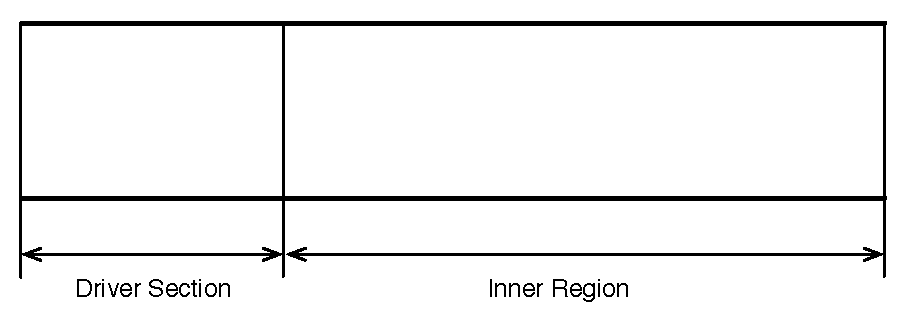
\includegraphics[width=9cm,clip]{Driver.eps}
\end{center}
\caption{ドライバセクションを含む流れ解析.}
\label{fig:Driver}
\end{figure}

%
\subsection{ドライバセクションにおける周期境界の実装}

\textbf{図\ref{fig:Driver_prdc}}にドライバセクションの取り扱いを示す.
ドライバセクションはインデクス\verb|i=1~ip|の領域で,流出部のインデクスが\verb|i=ip|である.
ドライバセクションの目的は,発達した流れを形成し,計算する内部領域へと導くことである.
その際に支配方程式を満たすことが重要となる.

外部境界に対する周期境界であれば,単に,ドライバセクションの前後で計算した物理量を相互に交換すればよい.
ここで注意すべき点は,セル\verb|ip,ip+1|は計算内点にあり,数値流束$f_{ip+1/2}$をドライバセクションと内部領域で一致させる必要があることである.
単にデータを交換することは難しく,例えば一旦物理量を待避させ,その間に周期処理を行い,その後待避した物理量を戻すという処理などが必要になる.
つまり,特殊な操作をしないと通常のステンシル型の計算スキームでは境界条件を実装しにくい.
この点は,処理の複雑さによる処理コストの増加と並列計算時には同期待ちを生じるため,演算性能の低下につながる.

\begin{figure}[htbp]
\begin{center}
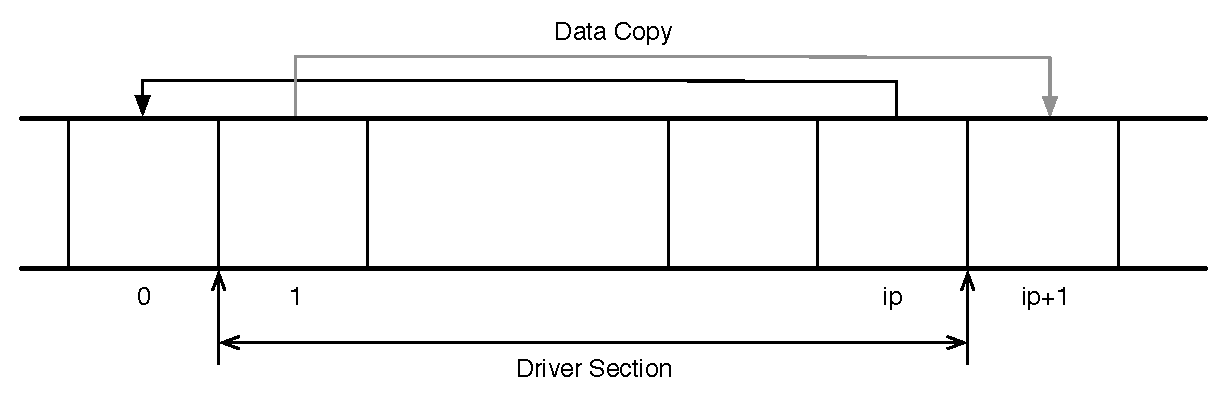
\includegraphics[width=13cm,clip]{Driver_prdc.eps}
\end{center}
\caption{ドライバセクションにおける周期境界処理.}
\label{fig:Driver_prdc}
\end{figure}

そこで,本来の目的に立ち返り,完全な周期境界でなく,あくまで流れを発達させることに重点をおき,なおかつ処理コストが低い方法を考える.
実装する方法は,以下のようになる.
\begin{itemize}
\item ドライバセクションでは,計算領域内部に用いる部分的な周期境界条件を実装する.
\item ドライバセクションの形状的な条件として,流入部と流出部の断面形状は同一で,座標軸に対して面直であること.必ず計算空間を構成する6面のどれかに接続していること.ドライバセクションは複数あっても良い.
\item 周期条件は,流出面から流入面へのone wayとする.計算は,ドライバセクションと内部領域にわたり,同じスキームにより計算する.このため,セル界面における数値流束は保存する.このとき,流入面へとコピーされる物理量は下流領域の影響を受けた値となるが,支配方程式を満たした値であるので,これを流入側に与えても問題はない.
\item ドライバセクションは圧力駆動とする.つまり,ドライバセクションの両端に圧力差を与え,速度はフリーとする\footnote{このため,計算内部領域の背圧によって流量が変化する可能性もある.その場合には,フィードバック機構を組み込み流量調整をする必要がある.}.
\end{itemize}

\subsubsection{速度}
速度の場合は,利用する空間スキームのステンシルに応じてデータをコピーする.

\subsubsection{圧力}
圧力の場合は,与える圧力差を$p_d$として,次式のように圧力値をコピーする.
\begin{equation}
p_0 \,=\, p_{ip} + p_d
\end{equation}

\subsubsection{パッシブスカラ}
非圧縮の温度のようなパッシブスカラ値については,ドライバセクション流出部の状況によらず,常に流入部で指定値を与える.


%
\subsection{ボクセルモデルの指定}
\textbf{図\ref{fig:Driver_voxel}}にドライバセクションを指定する場合のボクセルIDの例を示す.ドライバセクションの内部とは別のIDで出口断面を与える点に注意する.

\begin{figure}[htbp]
\begin{minipage}{.65\textwidth}
\begin{center}
\includegraphics[width=10cm,clip]{Driver_voxel.eps}
\end{center}
\end{minipage} \hfill
\begin{minipage}{.3\textwidth}
\begin{center}
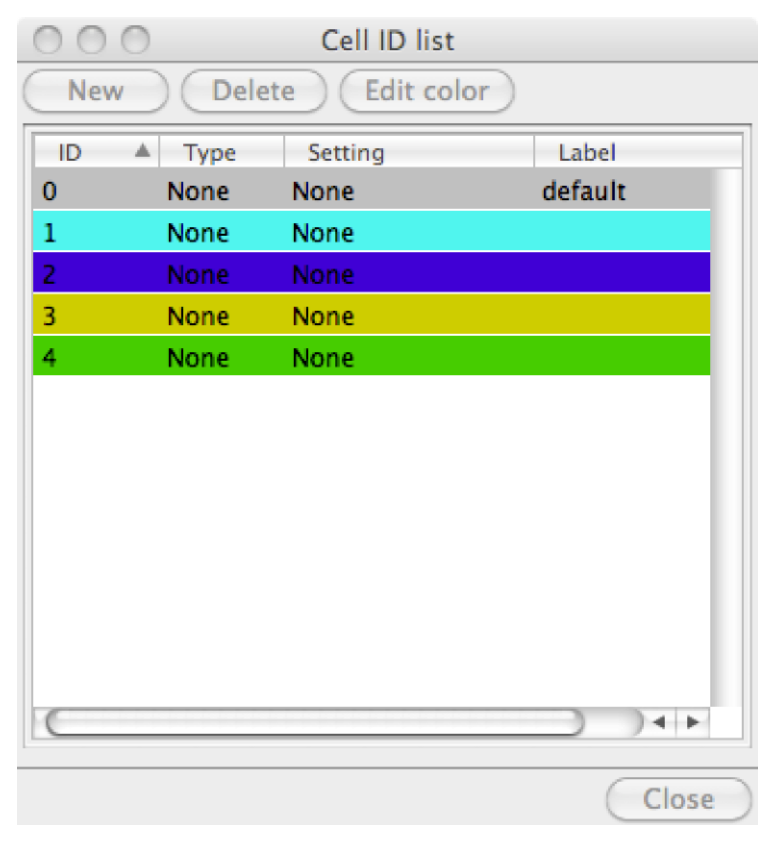
\includegraphics[width=5cm,clip]{Cell_id.eps}
\end{center}
\end{minipage}
\caption{チャネル流のボクセル設定.ID=1:内部流体,ID=2:固体セル,ID=3:ドライバセクション(流体),ID=4:ドライバセクションの流出断面(流体).}
\label{fig:Driver_voxel}
\end{figure}

%
\pagebreak
\subsection{境界の指定方法}
\textbf{図\ref{fig:Driver_voxel}}を例に,境界条件の指定方法を示す.
ドライバセクションを利用するためには,内部境界と外部境界の両方の指定が必要になる.

\subsubsection{内部境界}
{ \small
\begin{program}
<InnerBoundary>
  <Elem comment="inner_driver" id="4" name="Periodic">
    <Param dtype="STRING" name="Upstream_Direction"  value="X_minus"/>
    <Param dtype="REAL"   name="Pressure_Difference" value="1.636e-4"/>
    <Param name="def_face"  dtype="INT"  value="1" />
  </Elem>
</InnerBoundary>
\end{program}
}

内部境界で指定するUpstream\_Directionと外部境界で指定するDriver\_Directionの方向は同じであること.

\subsubsection{外部境界}

{ \small
\begin{program}
<OuterBoundary>
  <Elem id="10" name="Periodic">
    <Param dtype="STRING" name="Mode" value="Driver"/>
    <Param dtype="STRING" name="Driver_Direction" value="X_minus"/>
    <Param dtype="int"    name="Driver_Lid_Index" value="28"/>
  </Elem>
</OuterBoundary>
\end{program}
}

Driver\_Lid\_Indexには,流入方向の空間インデクス値を指定する.
この値がわからない場合には,適当な値をいれておき,CBCソルバを実行すると,コンポーネント情報の部分に下記のように表示されるので,その値を入力する.この例の場合には,X\_Minus方向がドライバの方向なので,i\_stの値を入力する.

{ \small
\begin{program}
>> Component Information

[Periodic]
 no            Label  ID  i_st  i_ed  j_st  j_ed  k_st  k_ed  Pressure Difference [Pa]/[-]  Driver
  1     inner_driver   4    28    28     2    29     2    29     1.63600e-04 / 3.21221e-01      X-
\end{program}
}

